\documentclass[12pt]{article}
\usepackage{longtable}
\usepackage{booktabs}
\usepackage{tabularx}
\usepackage{graphicx}
\usepackage{float}
\usepackage{fullpage}
\usepackage{longtable}
\usepackage{xltabular}
\usepackage{caption}
\usepackage{pdflscape}
\usepackage{afterpage}
\usepackage{multirow}
\usepackage[margin=1in]{geometry}
\usepackage{enumitem}

\newcounter{assumpnum} %Assumption Number
\newcommand{\atheassumpnum}{P\theassumpnum}
\newcommand{\aref}[1]{A\ref{#1}}
\newcounter{haznum} %Hazard Category Number
\newcommand{\hthehaznum}{H\thehaznum}
\newcommand{\href}[1]{H\ref{#1}}
\newcounter{srnum} %SR Number
\newcommand{\srthesrnum}{SR\thesrnum}
\newcommand{\srref}[1]{SR\ref{#1}}
\newcounter{fmeanum} %Table Counter
\newcommand{\fmeathefmeanum}{\thefmeanum}
\newcommand{\fmearef}[1]{\fmearef{#1}}

\title{Hazard Analysis\\\progname}

\author{\authname}

\date{}

%% Comments

\usepackage{color}

\newif\ifcomments\commentstrue %displays comments
%\newif\ifcomments\commentsfalse %so that comments do not display

\ifcomments
\newcommand{\authornote}[3]{\textcolor{#1}{[#3 ---#2]}}
\newcommand{\todo}[1]{\textcolor{red}{[TODO: #1]}}
\else
\newcommand{\authornote}[3]{}
\newcommand{\todo}[1]{}
\fi

\newcommand{\wss}[1]{\authornote{blue}{SS}{#1}} 
\newcommand{\plt}[1]{\authornote{magenta}{TPLT}{#1}} %For explanation of the template
\newcommand{\an}[1]{\authornote{cyan}{Author}{#1}}

%% Common Parts

\newcommand{\progname}{Mechatronics Engineering} % PUT YOUR PROGRAM NAME HERE
\newcommand{\authname}{Team 10, LiDart
\\ Jonathan Casella
\\ Karim Elmokattaf
\\ Michaela Schnull
\\ Neeraj Ahluwalia} % AUTHOR NAMES                  

\usepackage{hyperref}
    \hypersetup{colorlinks=true, linkcolor=blue, citecolor=blue, filecolor=blue,
                urlcolor=blue, unicode=false}
    \urlstyle{same}
                                


\begin{document}
\pagenumbering{roman}

\maketitle

\newpage

\tableofcontents
\listoffigures
\listoftables

~\newpage

\section*{Revision History}

\begin{tabularx}{1.0\textwidth}{p{3cm}p{2cm}p{4cm}X}
\toprule {\bf Date} & {\bf Version} & {\bf Authors} & {\bf Notes}\\
\midrule
10\textbackslash Oct\textbackslash 2022 & 1.0 & Michaela Schnull \newline Kareem Elmokattaf  & Initial Release\\
\bottomrule
\end{tabularx}

~\newpage

\section{Reference Material}

This section records information for easy reference.

\subsection{Abbreviations and Acronyms}

\renewcommand{\arraystretch}{1.2}
\begin{tabular}{l l} 
  \toprule		
  \textbf{Symbol} & \textbf{Description}\\
  \midrule 
  A & Assumption\\
  ALARA & As Low as Reasonably Achievable\\
  FMEA & Failure Modes and Effects Analysis\\
  GUI & Graphical User Interface\\
  H & Hazard\\
  SR & Safety Requirement\\
  \bottomrule
\end{tabular}\\

\pagenumbering{arabic}

\section{Background}

3D scanning is a versatile technology that is used across many industries, but its uses are often limited by high cost
and complexity. \progname aims to build a low cost, simple to use 3D scanning robot. A software suite will process
data obtained from the robot and provide a user interface. \progname’s end product will be a wheel based mobile robot
with all required sensors on-board that can be connected to over WiFi.

\section{Introduction}

\subsection{Purpose}

The purpose of this document is to identify and provide actions to eliminate or mitigate hazards associated with the setup and operation of \progname. This document is intended to identify failure modes, effects, and causes related to the safety of the system. Recommended actions have been assigned to each failure mode.

\subsection{Scope}
The \progname ~system consists of a graphical user interface that allows the user to remotely drive a robot, initiate 3D scans, and download the final stitched 3D scan. Hazard analysis will be performed on all processes relating to the installation and operation of the LiDart system.  Hazard analysis will not be completed for software components such as licensing, user authentication, security, and data storage as these considerations are not within the scope of the project. Failure modes due to human performance factors are not included in this hazard analysis.

\section{Assumptions and Definitions}

\subsection{Assumptions}

The following assumptions were used in the development of this process FMEA:

\noindent \begin{itemize}
\item[A\refstepcounter{assumpnum}\theassumpnum \label{Assumption1}:] The \progname ~system is in good condition. All maintenance activities have been properly completed. 

\item[A\refstepcounter{assumpnum}\theassumpnum \label{Assumption2}:]The \progname ~system has not been damaged or modified by the user.

\item[A\refstepcounter{assumpnum}\theassumpnum \label{Assumption4}:] The user will follow operating instructions as provided in the user manual.

\end{itemize}

\subsection{Definitions}

\subsubsection{Hazard}

The definition of a hazard used throughout this document is based on  Nancy Leveson's work. A hazard is defined as any property or condition of a system coupled with an environment that has the potential to cause harm, damage, or adverse effects.

\section{System Overview}

The \progname ~system is a 3D scanning solution in the form of a mobile robot. The system includes location markers, a remote-controlled robot, and a graphical user interface.

\subsection{System Boundary}

Hazard analysis is performed on \progname ~system, which consists of: 

\begin{itemize}
\item The physical robot, including the hardware and firmware running on the robot
\item Location markers
\item The GUI application
\item A WiFi network
\end{itemize}

The physical device running the GUI application and the environment surrounding the robot are not controlled by \progname. Hazard analysis will not be performed on elements external to the system.
 
\subsection{System Processes}

 \noindent The processes executed by the \progname ~system can be broken into the following categories:

\noindent \begin{itemize}
\item[\textbf{H\thehaznum \label{H0}}] \textbf{General Failure Modes}\\
Consists of the failure modes that may occur at any time. 

\item[\textbf{H\refstepcounter{haznum}\thehaznum \label{H1}}] \textbf{System Setup and Installation}\\
Before performing scanning operations, the robot must be powered on, and communication must be established between the robot and the user interface over WiFi. A series of functionality checks are performed after communication is established to ensure the robot is in an operational state. Furthermore, location markers must be installed. Figure~\ref{fig_Setup} illustrates the setup and installation processes.
\begin{figure}[H]
\centering 
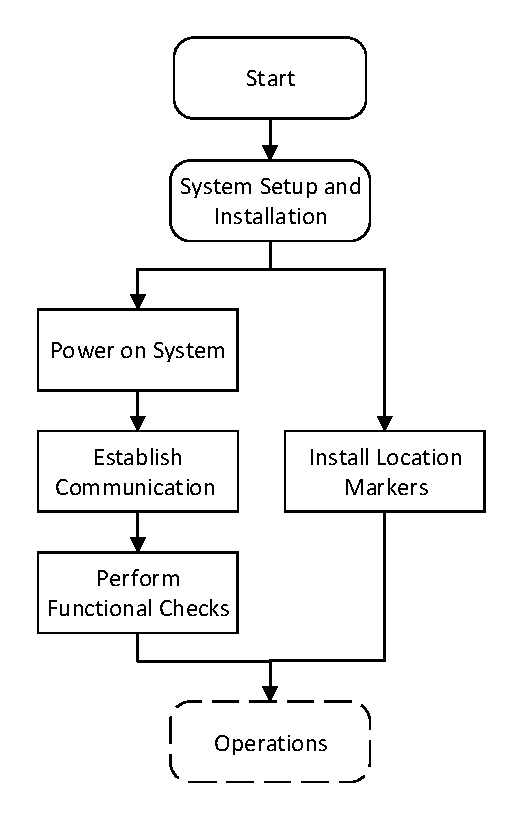
\includegraphics[width=0.5\textwidth]{Figures/Setup Processes.pdf}
\caption{Setup and Installation Process Diagram}
\label{fig_Setup}
\end{figure}

\item[\textbf{H\refstepcounter{haznum}\thehaznum \label{H2}}] \textbf{Operation}\\
While in operation, the robot must respond to inputs from the user and perform scanning operations. The system must perform state estimation, acquire sensor data, and output 3D models. Figure~\ref{fig_Operation} illustrates the operational process logic.
\begin{figure}[H]
\centering
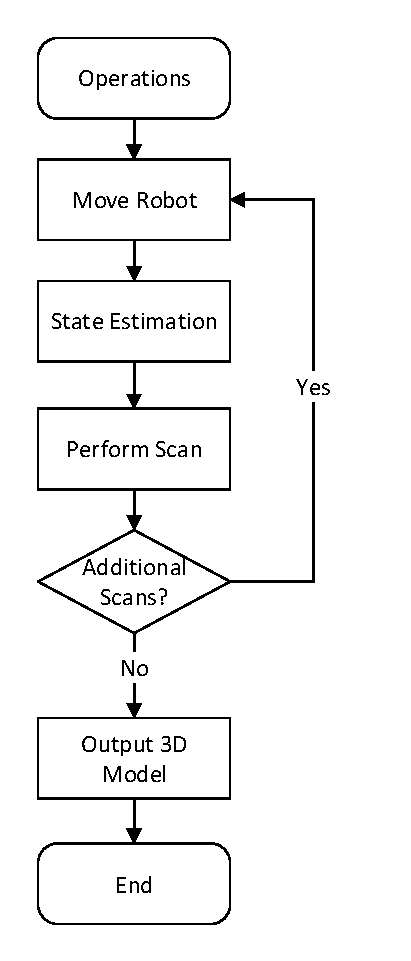
\includegraphics[width = 0.4\textwidth]{Figures/Operation Processes.pdf}
\caption{Operation Process Diagram}
\label{fig_Operation}
\end{figure}
\end{itemize}

\section{Failure Modes and Effects Analysis}

A Failure Modes and Effects Analysis (FMEA) is used to perform hazard analysis of the \progname ~system. The table is included in Appendix ~\ref{FMEA}.

\section{Recommended Actions and Safety Requirements}

\section{Roadmap }

New safety requirements created from the hazard analysis will improve the safety of the \progname ~system. Additionally, recommended actions from the FMEA will be implemented throughout the design phase of this project to eliminate and mitigate hazards. The principle of ALARA will be used to reduce risk and decide which recommended actions will be implemented. 


\afterpage{
\clearpage
\thispagestyle{empty}
\newgeometry{margin=0.5in}
\begin{landscape}
\centering
\appendix
\section{Failure Modes and Effects Analysis Table}
\label{FMEA}
\tiny
\captionof{table}{Failure Modes and Effects Analysis}
\begin{xltabular}{\linewidth}{|p{3cm}|p{1cm}|p{3.25cm}|p{3.25cm}|p{3cm}|p{3cm}|p{4cm}|X|}
\hline
\textbf{Design Component} & \textbf{Ref.} & \textbf{Failure Mode} & \textbf{Cause of Failure} & \textbf{Effect of Failure} & \textbf{Detection} & \textbf{Recommended Actions} & \textbf{SR}\\
\hline
\multicolumn{8}{|c|}{General Failure Modes}\\

\hline
Robot location calibration & H0-1& Robot can't calibrate its location & Robot can't start scanning & - Tags are not in visible range of the robot & Software checks for calibration confirmation & - Adjusting the placement of the tags to be visible by the robot & {}\\ %word it better
{} & {} & {} & {} & - Not enough tags are placed to calibrate the robot &  {} & - Ensuring enough tags are placed around the space & {}\\

\hline
GUI & H0-2 & GUI crashes & - Bugs in software due to memory management \newline - Performance issues & - Communication with robot is lost \newline - Robot continues to move after communication is lost \newline -Current scanning data lost & Visual inspection & - Provide auto-save feature \newline - Place the robot in safe-state if communication is lost & {}\\

\hline
System Power & H0-3 & Power is lost & - Damaged battery \newline - Battery died \newline - Short circuit & -Robot no longer functions and is completely halted & Visual inspection &- Charge the battery \newline - Replace the damaged battery \newline - Fix short circuit& {}\\

\hline
\multicolumn{8}{|c|}{System Setup and Installation}\\

%Establish Communication
\hline
Establish Communication & H1-1 & Cannot establish communication with robot & Network connectivity issue & Delay to investigate and fix network issues & {} & Reset the network \newline & {}\\

%Functional Checks

\hline
Functional Checks & H1-2 & Functional checks (e.g. check that ll required devices are connected) are not successful & - Checks fail when they should pass \newline - Checks pass when they should fail & Delay to investigate and fix error \newline Potential downstream functional and performance issues & {} & {}& {}\\

\hline
LiDar Sensor Calibration& H1-3 & Sensor doesn't scan the object & 3D scanning can't take place & LiDar Sensor hasn't been calibrated properly & Software checks for calibration confirmation from sensors & Following steps to calibrate the sensor & {}\\ %look at this again

\hline
\multicolumn{8}{|c|}{Operation}\\

%Communication
\hline
Communication & H2-1 & Communication between the GUI and the robot is lost & - Wifi signal is too weak \newline - WiFi signal intermittently cuts out & - Robot will not be able to be controlled by user \newline - Data messages are lost & Through GUI & - Keep the robot closer to the WiFi signal \newline - Use networking protocols that check for missed messages & {}\\

%Movement of robot
\hline
\multirow{2}{*}{Movement of Robot} & H2-2 & Robot crashes & - Robot does not respond to input \newline - Robot is not capable of stopping in time & - Damage to the surrounding environment & {} & - Display warning when the robot is getting too close to an obstacle \newline - Use software controls to prevent user input from instructing the robot to drive into an obstacle & {}\\\cline{2-8}
& H2-3 & Robot does not move as instructed by user input & Robot could end up in the wrong location & Communication strength not being strong enough (WiFi signals) & Software checks the strength of the signal between host and robot &Limiting robots movement to keep signal strength with the host & {}\\ %compare to other entry

\hline
\multirow{2}{*}{State Estimation}  & H2-4 & State cannot be estimated & - Markers are not in the camera(s)' field of view \newline - Camera cannot identify markers\newline -No encoder feedback \newline Inadequate number of markers & System cannot correctly perform scanning operations & Software checks for calibration confirmation & - Re-calibrate the system \newline - Ensure enough markers are used \newline - Adjust the position of markers so that they are visible to the robot \newline - Move the robot to a new location & {}\\\cline{2-8}
& H2-5 & False positive that the state is correctly estimated & State estimation filtering error & {} & {} & {}& {}\\\cline{2-8}
& H2-6 & False negative that state has not been correctly estimated & State estimation filtering error & {} & {} & {}& {}\\\cline{2-8}

%Perform Scan
\hline
\multirow{2}{*}{Perform Scan} & H2-7 & Incorrect amount of data acquired & Insufficient amount of data acquired & Accuracy of output may decrease  & {} & {}& {}\\\cline{2-8}
& H2-8 & Data acquired is not correct & - Sensor malfunction \newline - Robot moves during data acquisition & 3D models are inaccurate & {} & -Use software controls to prevent the robot from moving during scanning \newline - Validate output of sensor data& {}\\\cline{2-8}
\hline

\hline
{} & {} & {} & {} & {} & {} & {}& {}\\

\hline
{} & {} & {} & {} & {} & {} & {}& {}\\

\hline
{} & {} & {} & {} & {} & {} & {}& {}\\


\end{xltabular}
\end{landscape}
\clearpage% Flush page
}

\end{document}